% Intended LaTeX compiler: pdflatex
\documentclass[11pt]{article}
\usepackage[utf8]{inputenc}
\usepackage[T1]{fontenc}
\usepackage{graphicx}
\usepackage{longtable}
\usepackage{wrapfig}
\usepackage{rotating}
\usepackage[normalem]{ulem}
\usepackage{amsmath}
\usepackage{amssymb}
\usepackage{capt-of}
\usepackage{hyperref}
\author{Fethi Okyar}
\date{2026-02-18}
\title{Chapter 1: Introduction\\\medskip
\large Reading: [Fung/94] \href{../textbook\_excerpts/1\_TensorAlgebra.pdf}{Chapter 1}}
\hypersetup{
 pdfauthor={Fethi Okyar},
 pdftitle={Chapter 1: Introduction},
 pdfkeywords={},
 pdfsubject={},
 pdfcreator={Emacs 30.2 (Org mode 9.7.11)}, 
 pdflang={English}}
\begin{document}

\maketitle
\setcounter{tocdepth}{1}
\tableofcontents

\section*{(\(\S 1.1\)) Objectives (Session 1)}
\label{sec:org25212e7}
\begin{itemize}
\item To emphasize the formulation of problems in mechanics,
\item To reduce vague ideas into precise mathematical statements,
\item To cultivate the habit of questioning, analyzing, and designing,
\item To observe nature, think of previous problems, write down a possible set of governing equations and boundary conditions.
\end{itemize}
\subsubsection*{What is \emph{mechanics} concerned with?}
\label{sec:org9494286}
\begin{itemize}
\item Motion
\item Deformation
\item Flow
\item Force
\item Energy
\item Interactions
\item Internal changes
\item temporarily or permanently
\item reversibly or irreversibly
\end{itemize}

\begin{itemize}
\item These changes (deformation, etc.) together with axioms of continuum mechanics, can be expressed as boundary value problems
$$ \frac{\partial \sigma_{ij}}{\partial x_i} + f_j = \frac{\partial v_j}{\partial t}, \hspace{1em} \forall x \in \Omega $$
\begin{align}
 n_i \sigma_{ij} = \bar{t_j} \hspace{1em} & \forall x \in \partial\Omega_n \\
 u_i = \bar{u}_i \hspace{1em} & \forall x \in \partial\Omega - \partial\Omega_n
\end{align}

\item We will be dealing with fundamental principles that underlie these differential equations and their boundary conditions
\end{itemize}
\subsubsection*{Mechanics (definition)}
\label{sec:orgc715120}
\begin{center}
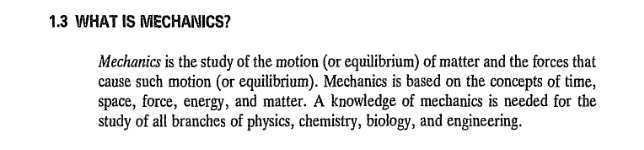
\includegraphics[width=.9\linewidth]{./images/FU94-SS-1.png}
\end{center}
\section*{(\(\S 1.4\)) Prototype of a Continuum}
\label{sec:org3d86e8c}
What is a \emph{Continuum}?
\begin{itemize}
\item good question\ldots{} ask chatGPT\\
\uline{PROMPT:} we are a group of undergraduate students enrolled in the biomedical engineering program. we are taking the biomechanics course, and it is the first time that we encounter the notion of a continuum. How could you give an everyday description of this cohort?
\item Is the real number system a \emph{continuum}?
\item What about matter occupying a volume in 3D space? What is the most obvious reason for not being able to call \textbf{matter} as a continuum?
\end{itemize}

\begin{center}
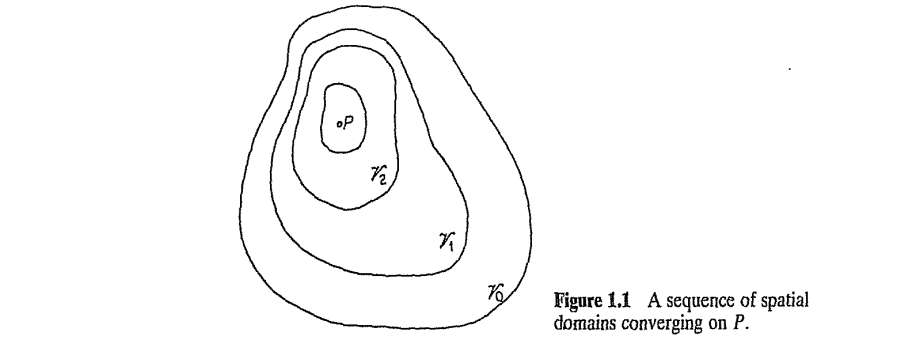
\includegraphics[width=.9\linewidth]{./images/FU94-fig1.1.png}
\end{center}
\begin{itemize}
\item We let the amount of matter be measured by \emph{mass} and assume matter permeates a certain space \(\mathcal{V}_0\)
\item We consider a point \(P\) in \(\mathcal{V}_0\) and a sequence of subspaces \(\mathcal{V}_1,\, \mathcal{V}_2,\, \ldots\), converging on \(P\):
$$ \mathcal{V}_n \in \mathcal{V}_{n-1}, \hspace{1em} P \in \mathcal{V}_n, \hspace{1em} \mathrm{(n=1,2,...)}. $$
\end{itemize}
\subsection*{Notion of Density, \(\rho\)}
\label{sec:orgf751610}
\begin{itemize}
\item Let the volume encapsulated in \(\mathcal{V}_n\) be denoted by \(V_n\) and the mass of the matter contained in \(\mathcal{V}_n\) be denoted by \(M_n\).
\item If the limit of \(m_n/V_n\) exists as \(n \to \infty\) and \(V_n \to 0\), the limiting value is defined as the \emph{density of the mass distribution} at the point \(P\), and is denoted by \(\rho(P)\):
$$ \rho(P) = \lim_{V_n \to 0} \frac{m_n}{V_n} $$
\item \emph{An ideal material continuum is a} definition for which \emph{the densities of mass, momentum and energy exist in this strict mathematical sense}.
\item But unfortunately no such materials exists!!
\end{itemize}
\subsection*{Modifying the Limit to fit Reality}
\label{sec:org5478816}
\begin{itemize}
\item As \(n \to \infty\), the limit of \(V_n\) tends to a finite positive number \(\omega\).
\item The volume is not let to vanish but tends to a non-zero value controlled by a characteristic size, e.g. on the order of \(\mathcal{O}(\mu m)\), below which the continuity and homogeneity of the distribution is disrupted.
\item The quantity \(\rho\) is then said to be the \emph{density of material at \(P\) with an  acceptable variability \(\epsilon\) in a defining limit volume \(\omega\)}.
\item This is ``\emph{our definition of a continuum}''.
\end{itemize}
\section*{(\(\S 1.6\)) Notion of Stress}
\label{sec:orgd752160}
The Scene:
\begin{itemize}
\item Consider a material \(B\) occupying a spatial region \(V\).
\item Imagine a closed surface \(S\) within \(B\) and consider the interaction between material separated by \(S\).
\item At a point \(P\) on \(S\), let the outward unit normal be \(\boldsymbol{n}\).
\item Consider a limited area on \(S\) around \(P\), called \(\Delta S\).
\item Material on the outer region are labeled as \(+\), while the opposite ones are \(-\).
\item Consider the total force exerted by the \(+\) side on the \(-\) side be represented by the force vector, \(\Delta \boldsymbol{F}\).
\item We define a limit (in the modified sense described above) of the ratio
$$\lim_{\Delta S \to 0} \frac{\Delta \boldsymbol{F}}{\Delta S} \triangleq \overset{(\boldsymbol{n})}{\boldsymbol{t}}$$
as the traction at point \(P\) over a plane with normal \(\boldsymbol{n}\).
\item Traction is also known as the stress vector, and is a measure of the amount of force passing thru a unit area.
\end{itemize}

\begin{center}
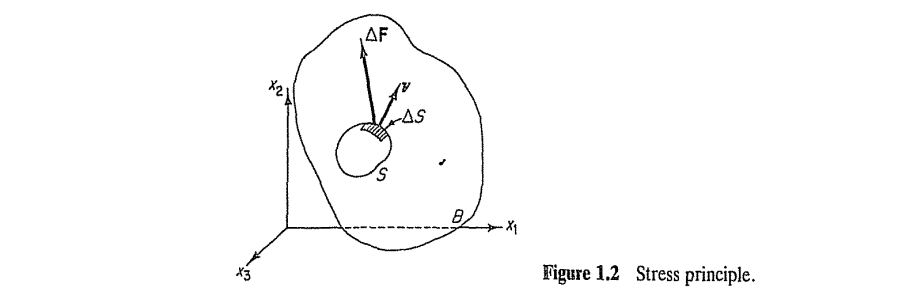
\includegraphics[width=.9\linewidth]{./images/FU94-fig1.2.png}
\end{center}

$$ \overset{(\boldsymbol{n})}{\boldsymbol{t}} = \frac{d \boldsymbol{F}}{d S} $$

The stress principle of Euler and Cauchy.
\section*{(\(\S 1.7\)) Abstract Copy of a Real Continuum}
\label{sec:orgef77cdd}
\begin{itemize}
\item Imagine we obtain the material properties (e.g. density, etc.) of a matter (real continuum).
\item To make useful calculations we need a mathematical model that uses these properties.
\item We say we clone the real material and produce an abstract copy of it.
\item This abstract copy is isomorphic with the real number system, it is an idealization.
\item Whereas the real material would have a limitation on the lower bound of sizes, the calculus of the idealized system can be carried out.
\item There may be a need to use more than one abstraction of the real material in a different range of sizes. The behaviour of a material in millimeter scale may be different from its behaviour in micron scale. This depends on the \emph{hierarchy} of material constitution.
\item More about hierarcy of the making of biological tissues in \(\S 1.10\).
\end{itemize}
\section*{(\(\S 1.9\)) Axioms of Continuum Mechanics}
\label{sec:orge95a203}
\begin{itemize}
\item First, the axioms of physics, i.e. the balance of momentum, the balance of moment of momentum, and the first and second laws of thermostatics are copied as axioms of continuum mechanics,
\item Second, \emph{a material continuum remains as a continuum under the action of forces}, i.e., the \emph{axiom of continuity}. This does not limit the opening of new surfaces due to fracturing or tearing, but these have to be accounted for in a thermodynamic sense. Also, growth (increase or migration of cells) or resorption (reduction) of matter is allowed,
\item Third, the stress and strain can be determined everywhere, which is the \emph{axiom of determinism}.
\item Fourth, the stress at a point depends on the strain at and around that point, the \emph{axiom of neighborhood},
\item Fifth, the stress at a given moment depends on the strain at that moment and and previous moments, the \emph{axiom of memory}. The stress-strain relation may be influenced by other parameters such as temperature, electrical change, ion transport, etc., that is the problem is of a multi-physics nature.
\end{itemize}
\section*{(\(\S 1.10\)) A Biological Example of Hierarchy of Continua}
\label{sec:org59c8ad8}
The change of microstructure by shifting the scale of observation (i.e. switching the scale of magnification of a microscope, x100, x10\(^4\), x10\(^6\), etc.). 

One example is the human lung. Three consecutive trees, an airway tree, an arterial three and a venous tree.
\begin{center}
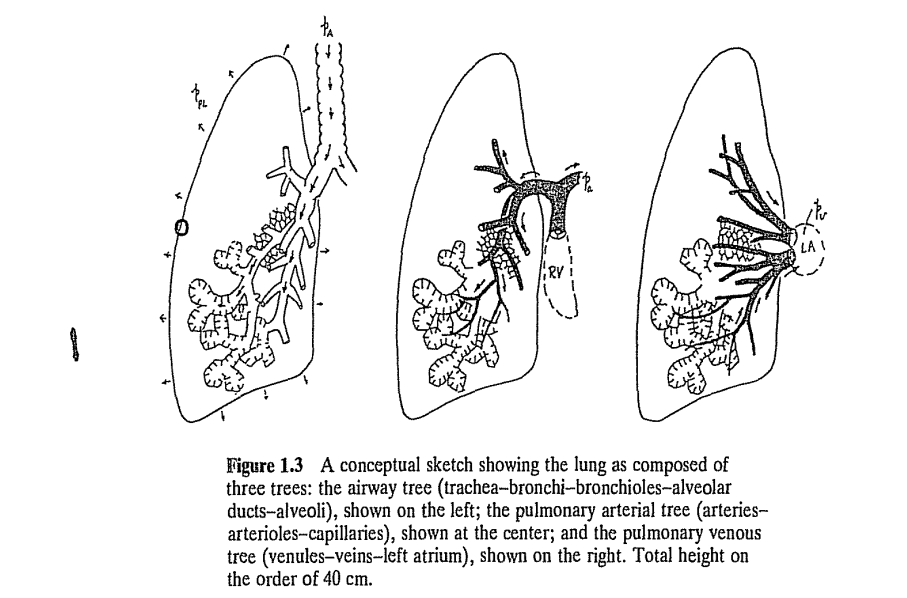
\includegraphics[width=.9\linewidth]{./images/FU94-fig1.3.png}
\end{center}

\begin{center}
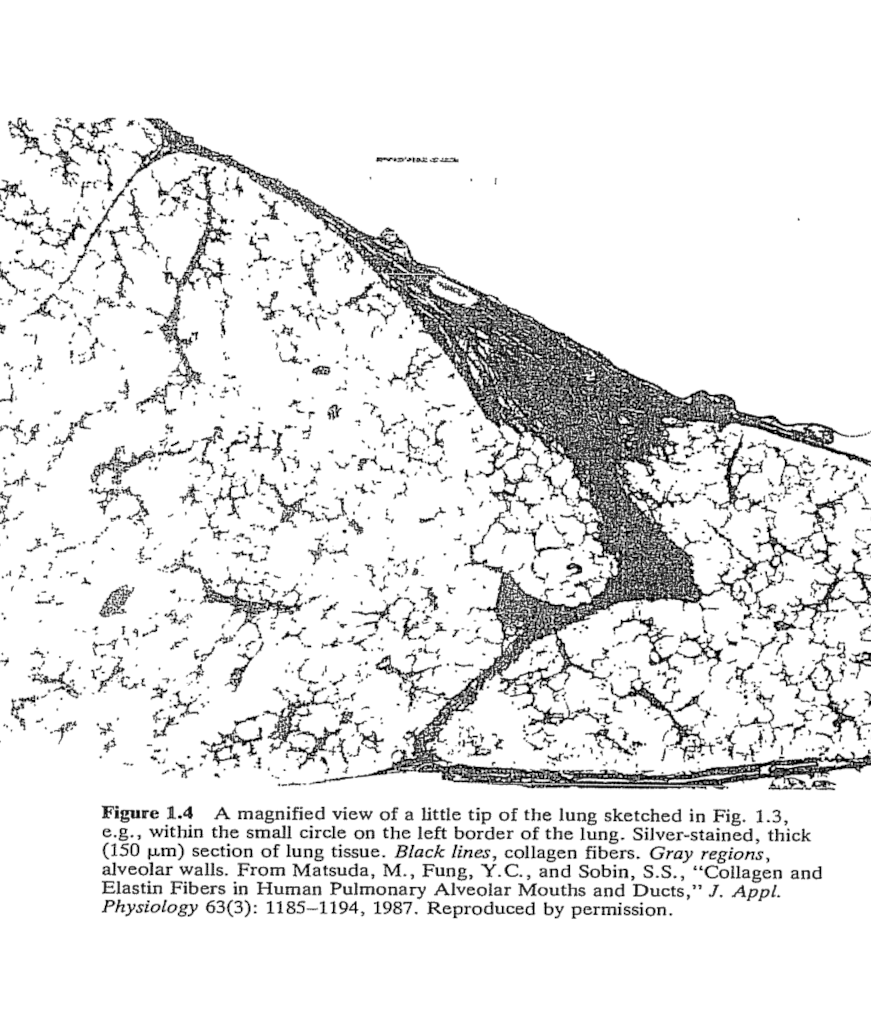
\includegraphics[width=.9\linewidth]{./images/FU94-fig1.4.png}
\end{center}

\begin{center}
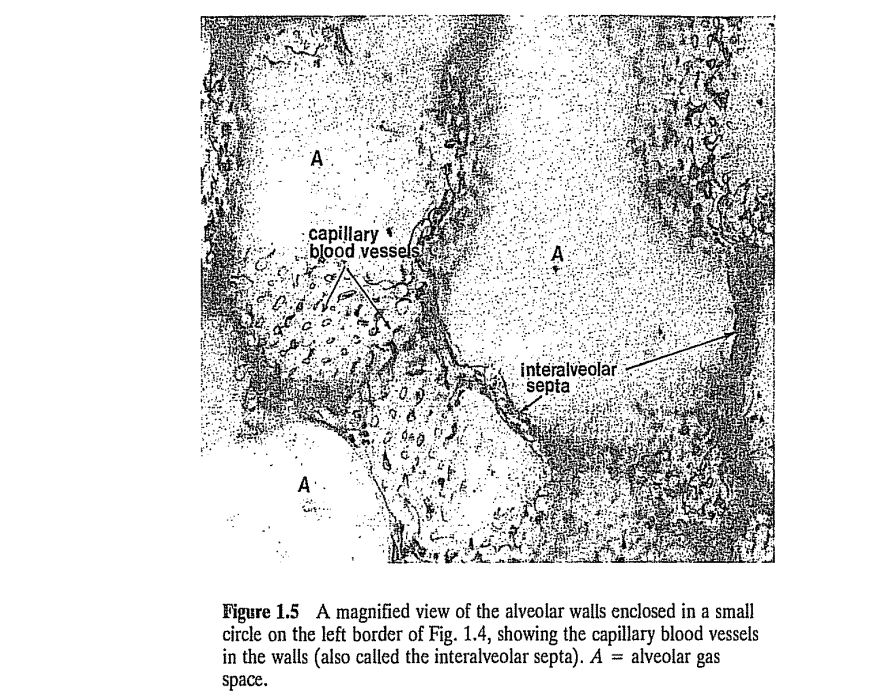
\includegraphics[width=.9\linewidth]{./images/FU94-fig1.5.png}
\end{center}
\subsection*{Questions for next session}
\label{sec:org27fa9f6}
Ask AI:
\begin{itemize}
\item Discuss the meaning of a free-body diagram in the context of mechanics.
\end{itemize}
\subsection*{Motivation}
\label{sec:orgc487876}
A recent post in Linkedin reveals the computational simulation of breathing.
\url{./images/breathing.gif}
\section*{(\(\S 1.11\)) Equations of Motion and Equilibrium}
\label{sec:orgc08c4b9}
\subsection*{Fundamentals}
\label{sec:org586161c}
\begin{itemize}
\item Let a body \(B\) occupy a region \(\mathcal{V}\) in space. We bring in calculus to calculate certain quantities such as the volume \(V\) enclosed in space \(\mathcal{V}\) as
$$ V = \int_\mathcal{B} dV $$
where the integral is taken over the entire body which implies that \(\int\) is synonymous with a triple integral, and \(dV\) represents a three-dimensional volume element (e.g. \(dV=dx\,dy\,dz\) in cartesian coordinates).
\item The notion of a coordinate system enters into our treatment as a tool for locating points in space. We need as many rulers in a sense as the number of dimensions, \(n\),  in encapsulated by \(\mathcal{V}\). A three-dimensional coordinate system, for example, is set up by establishing its' origin \(O\) and three independent directions for measurement (i.e. \(x\), \(y\) and \(z\) directions, and their unit vectors \(\boldsymbol{i}\), \(\boldsymbol{j}\), and \(\boldsymbol{k}\)).
\item Note that there always is a reference of a reference, including our newly formed coordinate system \(O-xyz\).
\end{itemize}

\begin{itemize}
\item An important property of volume, as a geometric entity, is that it possesses a centroid, \(G\). The location of \(G\) can be determined by making use of the first moments of the volume integral with respect to three independent planes.
\item By the first moment we mean appending the differential element with its distance to a particular plane, for example, the first moment of the volume integral with respect to the \(x\) plane (i.e. the plane perpendicular to \(x\), or the \(y-z\) plane) would be
$$ \mathbb{1}_x(V) = \int_\mathcal{B} x dV $$
\item For example, the \(x\) coordinate of the centroid can then be determined by evaluating
$$ x_G = \frac{\mathbb{1}_x(V)}{V} $$
The other two coordinates can be found by applying a similar procedure for the \(y\) and \(z\) planes.
$$ y_G = \mathbb{1}_y(V)/V,\hspace{1em} z_G = \mathbb{1}_z(V)/V $$
\end{itemize}

\begin{itemize}
\item If the mass density of matter filling this space is given as \(\rho(\boldsymbol{x})\), where it is assumed that the density field is a function of the location, we can use it to calculate the mass \(m\) of \(\mathcal{B}\) by introducing density into the above integral,
$$ m = \int_\mathcal{B} \rho(\boldsymbol{x}) dV $$
Here the location symbol \(\boldsymbol{x}\) represents the three coordinates of the differential element grouped in a vector form (a list of ordered numbers) as \(\boldsymbol{x} = \{x,\,y,\,z\}\). Usually the functional dependence of \(\rho\) on \(\boldsymbol{x}\) is not indicated explicitly for the purpose of mathematical brevity, i.e. we write
$$ m = \int_\mathcal{B} \rho dV $$
\end{itemize}

\begin{itemize}
\item We accept that the axioms of the \emph{balance of momentum} and \emph{balance of moment of momentum} govern motion of bodies under forces. (Tested positive against experimental findings for almost about the past 400 years.)
\item Bodies reduce to particles when their scale is dominated by the effect of the force acting upon them. Then we simply call the body as a \emph{point mass} or a \emph{particle}.
\item In that case, the body becomes distant and its \emph{shape} and \emph{orientation} becomes immaterial to the problem at hand. Its effectively treated by tracking its centoid, \(G\).
\item Having left its ``cover and shape'', a body is only able to receive external forces from its centroid, whence the concept of \emph{moment of a force} acting upon this body also becomes immaterial.
\begin{center}
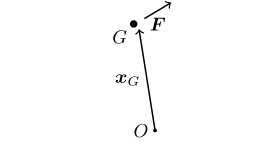
\includegraphics[width=.9\linewidth]{./images/fig1.11.1.png}
\end{center}
\item Remember that the moment, \(\boldsymbol{M}^O\), produced by a force, \(\boldsymbol{F}\), about point \(O\) can be determined by
$$ \boldsymbol{M}^O = \boldsymbol{r} \times \boldsymbol{F} $$
where \(\times\) denotes the vector (cross) product operation and \(O\) can be any arbitrary point in the theater.
\end{itemize}
\subsubsection*{Motion of a Body}
\label{sec:org52107cf}
\begin{itemize}
\item Let the body \(\mathcal{B}\) be traveling in curvilinear motion (without rotation) in space \(\mathcal{V}\). In this case, the time rate of change of point locations, \(\boldsymbol{x}\), in \(\mathcal{B}\) measured from an \emph{inertial frame of reference}
$$ \frac{d \boldsymbol{x}}{dt} \triangleq \boldsymbol{v} $$
are uniform, i.e. all points within are traveling with the same velocity,  \(\boldsymbol{v}\).

Freehand depiction of a body in curvilinear motion (i.e. moving with uniform velocity without rotation).

\item The time rate of change of velocity
$$ \frac{d \boldsymbol{v}}{dt} \triangleq \boldsymbol{a} $$
is called the acceleration of point \(\boldsymbol{x}\).

\item An inertial frame of reference is one which has no motion or one that moves with a constant velocity (zero acceleration).
\end{itemize}
\subsubsection*{Momentum of a Body (\textbf{24.02 mark})}
\label{sec:org3de5efc}
\begin{itemize}
\item The momentum of a body can be found by using a procedure similar to that used in determining its mass, i.e. integration
$$ \mathcal{P} = \int_\mathcal{B} \boldsymbol{v} \rho dV .$$
Here, \(\mathcal{P}\) is known as the \emph{linear momentum} or simply the \emph{momentum} of \(\mathcal{B}\).
\item For bodies in curvilinear translation, the velocity can be taken out of the integral due to its uniform nature (i.e. does not depend on the location in \(\mathcal{B}\)). Hence,
$$  \mathcal{P} = \boldsymbol{v} \int_\mathcal{B} \rho dV = m \boldsymbol{v}. $$
\item The moment of momentum (a.k.a \emph{angular momentum}) of the body can be expressed by introducing the moment operation into integration in the form of the vector product with the position vector from the point about which moment is taken, \(O\) for example
$$ \mathcal{H}^O = \int_\mathcal{B} \boldsymbol{r} \times \boldsymbol{v} \rho dV $$
\end{itemize}
\subsection*{Newton's, Euler's and/or Cauchy's Equations of Motion}
\label{sec:orga3a3495}
\begin{itemize}
\item States that: For ``the free-body or group of bodies'' isolated by replacing the effect received from their surroundings with corresponding force vectors, the net resultant of all external forces is equalized by the time rate of change of the group's momentum.
\item This can be interpreted in various ways. For example, the momentum will be preserved (it will not change) if the net resultant of the external forces is null (zero). (Newton's first law)
\item Another way to interpret this is by writing the mathematical statement
$$ \frac{d}{dt}m\boldsymbol{v} = \boldsymbol{F} $$
where \(\boldsymbol{F}\) is the net resultant force. This can be rewritten as
$$ m\boldsymbol{a} = \boldsymbol{F}. $$
\item Or still another way to write it is
$$  \boldsymbol{F} + (-m\boldsymbol{a}) = \boldsymbol{0}. $$
The paranthesized quantity is known as the \emph{inertial force} of D'alambert.
\end{itemize}
\subsubsection*{A Group of Particles}
\label{sec:orgd76a901}
\begin{itemize}
\item Whether it is a single particle or a group (system) of particles, we can isolate the mechanical effect of their surroundings by using the force hypothesis. We hypothesize that the external effect of the surroundings can be replaced with force vectors.
\item Say we have a group of \(K\) particles, and the superscript index \(I\) denotes the \(I\) th particle, \(m^I\) having an instantaneous velocity \(\boldsymbol{v}^I\).
\item We may establish the following set of logical rules about forces:
\begin{itemize}
\item Let \(\boldsymbol{F}^{IJ}\) denote the force of interaction exerted by \(J\) on \(I\), and \(\boldsymbol{F}^{JI}\) denote that of \(I\) on \(J\).
\item According to Newton's third, we can write
$$ \boldsymbol{F}^{IJ} = -\boldsymbol{F}^{JI} $$
\item When \(I==J\), i.e., the self-effected force onto itself \(\boldsymbol{F}^{II} = 0\).
\item The net force on particle \(I\), \(\boldsymbol{F}^{I}\) consists of the resultant force member \(I\) receives from other members \(J\), \(\sum_{J=1}^K \boldsymbol{F}^{IJ}\), and the force it directly receives from the surroundings, \(\overset{\mathrm{ex}}{\boldsymbol{F}^I}\).
\end{itemize}
\end{itemize}
\subsubsection*{The Equations of Motion for a Particle Group}
\label{sec:org6fedd2f}
\begin{itemize}
\item Thus the net force on particle \(I\) becomes
$$ \boldsymbol{F}^{I} = \overset{\mathrm{ex}}{\boldsymbol{F}^I} + \sum_{J=1}^K \boldsymbol{F}^{IJ} $$
\item The equation of motion of the \(I\) th particle becomes
$$ \frac{d}{dt} m^I\boldsymbol{v}^{I} = \overset{\mathrm{ex}}{\boldsymbol{F}^I} + \sum_{J=1}^K \boldsymbol{F}^{IJ}, \hspace{1.5em} (I = 1,2,\ldots,K) $$
\item If each particle has such an equation, \(K\) equations can be written corresponding to \(K\) particles in order to describe the motion of the group.
\item To be able to proceed with the solution, something about the nature of the mutual forces (\(\boldsymbol{F}^{IJ}\)) has to be known. This will be called as the \emph{constitutive properties} of the material system.
\end{itemize}
\subsubsection*{Equilibrium of Forces}
\label{sec:org1b7ef27}
\begin{itemize}
\item Describes the condition or state of motionlessness (have a zero net velocity). When a free-body or a group of bodies that are under the action of external forces is in equilibrium, the time rate of change of momentum vanishes and \emph{equations of motion} are renamed as \textbf{\emph{equations of equilibrium}}.
$$ \boldsymbol{0} = \overset{\mathrm{ex}}{\boldsymbol{F}^I} + \sum_{J=1}^K \boldsymbol{F}^{IJ}, \hspace{1.5em} (I = 1,2,\ldots,K) $$
\item Upon summing this equation over all particles \(I\) from 1 to \(K\), we obtain
$$ \sum_{I=1}^K \overset{\mathrm{ex}}{\boldsymbol{F}^I} + \sum_{I=1}^K  \sum_{J=1}^K \boldsymbol{F}^{IJ} =  \boldsymbol{0} $$
\item But the second term on the left hand side drops due to Newton's third law (internal forces are equal and opposite to one another) and we get the equation of equilibrium
$$ \sum_{I=1}^K \overset{\mathrm{ex}}{\boldsymbol{F}^I} =  \boldsymbol{0} $$
which states that \emph{for a body to be in equilibrium, the summation of all external forces acting on it is zero}.
\end{itemize}

\begin{itemize}
\item Equilibrium of forces is necessary and sufficient for the centroid of the body (or group of bodies) to remain steady (motionless), but does it guarantee total motionlessness?
\end{itemize}
\begin{itemize}
\item The answer is in the below figure. The external forces on a body (or group of bodies) may add up to a zero resultant force, however, the given force system may have a non-zero resultant moment.
\item The two forces, \(\boldsymbol{F}\) and \(\boldsymbol{-F}\) in the below figure form a ``couple''. A couple is a moment, \(\boldsymbol{M}\), formed by the system of two equal and opposite forces that are not collinear. The magnitude, \(M\), of the moment is equal to \(FD\), where \(F\) is the magnitude of \(\boldsymbol{F}\) and \(D\) is the shortest distance between their lines of action.

\begin{center}
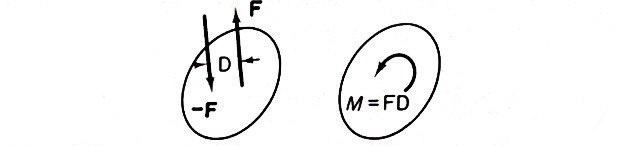
\includegraphics[width=.9\linewidth]{./images/FU77_fig1.2bc.jpg}
\end{center}
\end{itemize}

\begin{center}
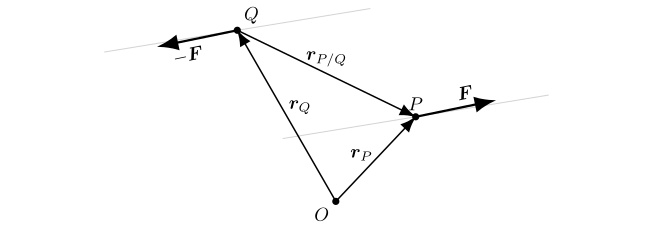
\includegraphics[width=.9\linewidth]{./images/fig1.11.2.jpg}
\end{center}
\begin{itemize}
\item The couple (moment) vector can be obtained by taking the summation of the moments of the couple about an arbitrary point \(O\). This results in
$$ \boldsymbol{M} = \boldsymbol{r}^{P/Q} \times \boldsymbol{F} $$
\item The system of couple forces vectors are said to be equivalent to their couple moment vector in terms of the mechanical effect produced on the body.
\end{itemize}
\subsubsection*{Equivalence of Force Systems}
\label{sec:orgbf5a2ad}
\begin{itemize}
\item We may be interested to simplify the force system acting on a body without changing the mechanical effect it produces.
\item For example, the forces may be repositioned to a common location in order to reduce them to a single force.
\item However, the repositioning of a force away from its line of action requires a careful process in order to maintain the overall mechanical effect produced by that force. See the figure below.

\begin{center}
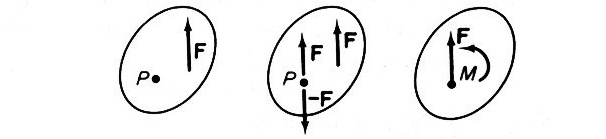
\includegraphics[width=.9\linewidth]{./images/FU77_fig1.2de.jpg}
\end{center}
\end{itemize}
\subsubsection*{Equilibrium of Moments}
\label{sec:orgf6e7115}
\begin{itemize}
\item The second condition of equilibrium of a free-body or group of bodies is derived based on the equilibrium of moments.
\item This requires that in addition to the equilibrium of forces derived previously, the external forces acting on the body should obey
$$ \sum_{I=1}^K \boldsymbol{r}^I \times \overset{\mathrm{ex}}{\boldsymbol{F}^I} =  \boldsymbol{0} $$
where \(\boldsymbol{r}^I\) denotes the position vector of particle \(I\) with respect to the origin \(O\) or any arbitrary location, \(Q\), for that matter.
\item The two equilibrium conditions are necessary and sufficient for a rigid body to remain motionless.
\end{itemize}

Example:
\url{https://emweb.unl.edu/negahban/em223/note11/note11.htm}

write an example script in \href{https://www.mathworks.com}{Matlab online} that calculates the resultant force and resultant moment of three external forces applied to a free-body

END OF UNIT 1
\end{document}
